\section{预备知识}
\label{sec:preliminary}


\subsection{检索头与稀疏头}
\label{subsec:attn_mechanism}

\paragraph{检索头与 FA}
检索头是一类专门从长序列中捕获上下文相关 token 的注意力头，使现代 LLM 能够有效处理长上下文任务~\citep{wu2024retrieval}。
在实践中，检索头通常采用标准全注意力（FA）计算模式。
给定 Query（$Q$）、Key（$K$）与 Value（$V$）状态，FA 的计算为：
\begin{equation}
\mathcal{O}_{r}=\mathrm{Softmax}\!\left(QK^{\top}\right)V,
\label{equ:dot_attention}
\end{equation}
其中为简化表达，省略了缩放因子。

\paragraph{稀疏头与 SA}
与检索头相比，稀疏头通过采用 SA 模式降低计算成本，仅保留最相关的一部分 $K$ 与 $V$（例如仅保留 20\% 的 key/value 状态）。
SA 的计算可定义为：
\begin{equation}
\mathcal{O}_{s}=\mathrm{Softmax}\!\left(Q\tilde{K}^{\top}\right)\tilde{V},
\label{equ:sparse_attention}
\end{equation}
其中 $\tilde{K}$ 与 $\tilde{V}$ 分别是 $K$、$V$ 的子集。

\paragraph{混合头机制}
尽管 SA 能显著降低计算量，但其可能引入性能下降~\citep{lu2025moba}。
为平衡效率与性能，近期方法提出在同一模型中混合检索头与稀疏头的 \emph{hybrid heads} 设计~\citep{xiaoduoattention2025,yu2025sliding,bhaskar2025cache}。
具体地，对于一个包含 $\mathrm{L}$ 层、每层有 $\mathrm{H}$ 个 key--value 头的 Transformer\footnote{此处采用 grouped query attention（GQA）~\citep{ainslie2023gqa} 的定义而非 multi-head attention（MHA），因为 GQA 在现代 LLM 架构中更常见。}，第 $\ell$ 层第 $h$ 个头被分配计算类型：$\pi^{(\ell, h)} \in \{\text{FA}, \text{SA}\}$，该层最终输出（$\mathbf{O}^{(\ell)}$）可写为：
\begin{equation}
\left\{
\begin{aligned}
& \mathbf{O}^{(\ell)} =
\mathrm{Concat}\!\left(
\mathcal{O}^{(\ell,1)},
\mathcal{O}^{(\ell,2)},
\dots,
\mathcal{O}^{(\ell,\mathrm{H})}
\right),\\
& \mathcal{O}^{(\ell,h)} =
\begin{cases}
\mathcal{O}_{r}, & \pi^{(\ell, h)}=\text{FA},\\
\mathcal{O}_{s}, & \pi^{(\ell, h)}=\text{SA},
\end{cases}
\end{aligned}
\right.
\label{equ:hybrid_concat}
\end{equation}


\begin{figure}[t]
  \centering
    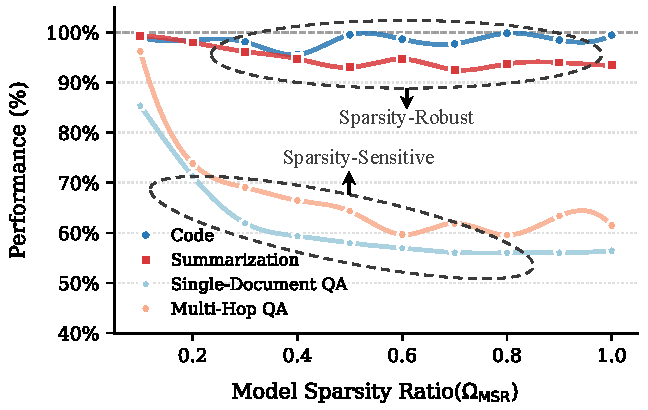
\includegraphics[width=\linewidth]{figures/per_task_performance_1.pdf}
     \caption{当混合模型稀疏率（$\mathbf{\Omega_{MSR}}$）提升时的性能变化趋势。性能以相对 FA 的百分比形式报告。}
  \label{fig:per_task_performance}
\end{figure}

\begin{figure*}[t]
\centering
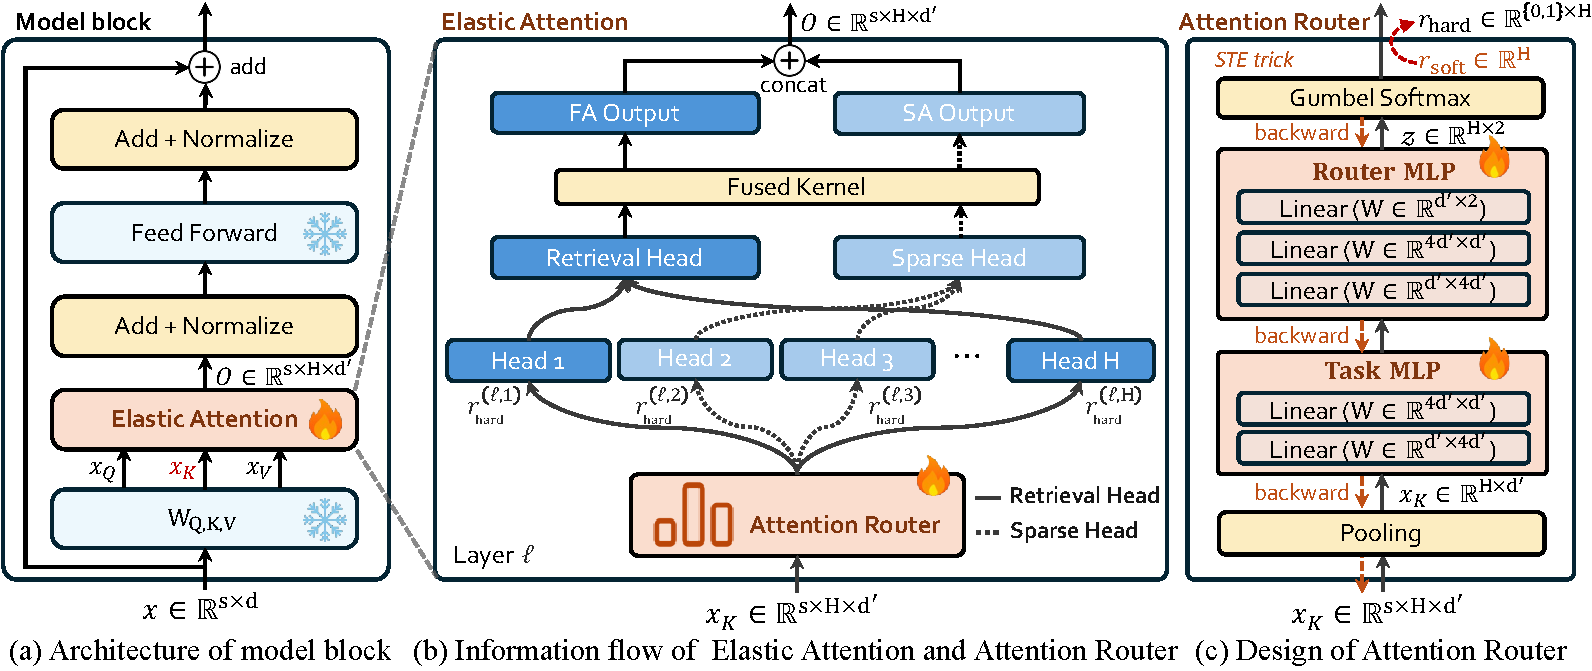
\includegraphics[width=0.95\linewidth]{figures/method_main.pdf}
\caption{我们提出的 Elastic Attention 示意图。(a) 为冻结骨干参数后的模型块；(b) 展示通过 Attention Router 动态分配头；(c) 给出 Attention Router 的轻量化结构。}
\label{fig:method_main}
\end{figure*}

\paragraph{稀疏率计算}
在混合头机制下，给定模型 $f_{\theta}$，我们从两个视角定义两种模型稀疏率：
（1）稀疏注意力头占比；（2）这些头实际关注 token 的比例。

\begin{definition}[模型稀疏率，$\Omega_{\mathrm{MSR}}$]
$\mathbf{\Omega_{\mathrm{MSR}}}$ 衡量模型中稀疏头所占比例：
\begin{equation}
\Omega_{\mathrm{MSR}}(f_{\theta})
= \frac{1}{\mathrm{H}}\frac{1}{\mathrm{L}}
\sum_{h=1}^{\mathrm{H}}\sum_{l=1}^{\mathrm{L}}
\mathbb{I}\!\left[\pi^{(\ell, h)}=\mathrm{SA}\right],
\end{equation}
其中 $\mathbb{I}[\cdot]$ 为指示函数。
\end{definition}

\begin{definition}[有效稀疏率，$\Omega_{\mathrm{ESR}}$]
$\mathbf{\Omega_{\mathrm{ESR}}}$ 衡量整个模型的有效稀疏程度，同时考虑稀疏头比例与其具体稀疏模式。其计算为：
\begin{equation}
\Omega_{\mathrm{ESR}}(f_{\theta})
=
\frac{1}{\mathrm{H}}
\frac{1}{\mathrm{L}}
\sum_{h=1}^{\mathrm{H}}
\sum_{\ell=1}^{\mathrm{L}}
\rho^{(\mathrm{\ell}, h)},
\end{equation}
其中 $\rho^{(\ell, h)} \in [0,1)$ 表示每个头的剪枝率；若头采用 FA，则 $\rho^{(\ell, h)}=0$（无 token 被剪枝）；若头采用 SA，则 $\rho^{(\ell, h)}=\rho_{\mathrm{SA}}$\footnote{不同 SA 策略对应不同 $\rho_{\mathrm{SA}}$。例如 SA 仅关注序列维度上 10\% token 时，$\rho_{\mathrm{SA}}=0.9$，表示 90\% token 被剪枝。}。
\end{definition}

\subsection{$\mathbf{\Omega_\mathrm{MSR}}$ 对下游任务的影响}
\label{subsec:deployment_sparisity}
尽管现有混合头机制在性能-效率上取得了较好权衡，但仍存在关键局限：\emph{$\mathit{\Omega_\mathit{MSR}}$ 在推理时固定不变，且其与下游任务性能的关系尚未被系统探索。}
本节研究不同 $\Omega_\mathrm{MSR}$ 取值对下游任务的影响。

\paragraph{设置}
我们使用 Llama3.1-8B-Instruct~\citep{grattafiori2024llama}，并遵循 \citet{wu2024retrieval} 的方法识别模型中的检索头并按激活频率排序。
基于该排序，我们逐步将检索头替换为稀疏头，从而提高 $\Omega_\mathrm{MSR}$。
我们在 LongBench~\citep{bai2024longbench} 上评估该过程产生的模型；该基准包含 6 类长上下文下游任务。
对不同 $\Omega_\mathrm{MSR}$，我们报告相对于骨干模型（全 FA）的性能百分比。
例如，当 $\Omega_\mathrm{MSR}=20\%$ 时，模型可能达到骨干模型（$\Omega_\mathrm{MSR}=0\%$）性能的 73.85\%。
关于检索头识别背景与实现细节见附录~\ref{appendix:preliminary_settings}。

\paragraph{结果}
如图~\ref{fig:per_task_performance} 所示，任务可大致划分为两类。
第一类为 \emph{\textbf{稀疏鲁棒型任务}}，其性能对 $\Omega_\mathrm{MSR}$ 变化不敏感。
这类任务通常仅需较粗粒度上下文信息即可完成，例如摘要。
第二类为 \emph{\textbf{稀疏敏感型任务}}，当 $\Omega_\mathrm{MSR}$ 超过某阈值后性能会快速下降。
这类任务通常需要从上下文中检索细粒度证据以给出准确输出，问答任务即为典型。
因此，\emph{无论任务类型数量多少，都可映射到上述两类之一}。
在该设定下，模型只需判断任务是否需要细粒度信息，并据此采用相应注意力计算模式。
